\section{Historical overview}

\begin{frame}{}
  \begin{itemize}[<+->]
    \item Bjerknes 1904
    \item Richardson 1922
    \item Charney, Fjørtoft, von Neumann 1950
    \item Rossby 1954
    \item Charney/U.S. Weather Bureau 1955
    \item Shuman 1966
    \item 1990
  \end{itemize}

\note<1>{
* Vilhelm Bjerknes 1904

Formulates weather forecasting as an initial-value
problem.

If it is true, as every scientist believes, that subsequent states of the
atmosphere develop from the preceding ones according to physical laws, then it
is apparent that the necessary and sufficient conditions for the rational solution
of forecasting problems are as follows.

— Sufficiently accurate knowledge of the state of the atmosphere
— Sufficiently accurate knowledge of the laws according to which one state
develops from another.

Primitive equations = Euler equations for non-viscous fluid + hydrostatic approx

}

\note<2>{
* Lewis Fry Richardson 1922

First numerical integration of the primitive equations.
Where he calculated change in surface pressure by hand.

Integrated the full primitive equations.
200x200 km grid with 4 vertical layers.
This took him many years.
Predicted a change of 146 hPa in just a few hours.
Close to no change in the measurements.

Led to many believing that numerical weather prediction was not possible.
}

\note<3>{
* Charney, Fjørtoft, von Neumann 1950

First numerical weather prediction using an electronic Computer.

ENIAC:
(the Electronic Numerical
Integrator and Computer),

One day integration of the Barotropic vorticity conservation equation.
Filters Inertia-gravity waves
Assume horisontal wind non-divergent.

The calculating speed of ENIAC was too slow for real time forecasting.
Hindcast, but very promising, no blowups like richardsons calculations.
}

\note<4>{
  Carl-Gustaf Rossby - Real time numerical weather prediction in Sweden

  Using the more powerful computer BESK.

}

\note<5>{
* 1955 - Three level quasigeostrophic model - U.S. Weather Bureau.

  Not used by forecasters until improvements were made in 1963.
}
\note<6>{
* 1966 - 6 layer model, 380x380 km grids.
Using the full primitive equations.

}

\note<7>{
* 1990 - Non hydrostatic models on smaller domains using full euler equations

}

\end{frame}

\begin{frame}{Today}

  \begin{table}[]
  \begin{tabular}{|l|l|l|ll}
  \cline{1-3}
  Organization & Grid size (km) & Vertical levels &  &  \\ \cline{1-3}
  NOAA         & 13x13          & 64              &  &  \\ \cline{1-3}
  UM           & 10x10          & 70              &  &  \\ \cline{1-3}
  ECMWF        & 9x9            & 137             &  &  \\ \cline{1-3}
  \end{tabular}

  \parencite{nwp}
  \end{table}

\end{frame}



\note{
    Examples of global models


}

\begin{frame}{Skill progress}
  \begin{figure}[H]
    \centering
    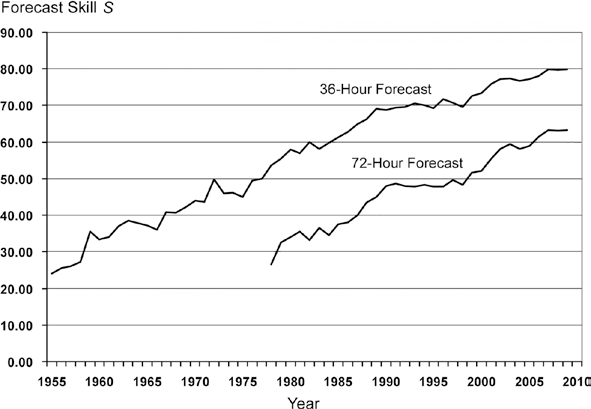
\includegraphics[width=0.8\textwidth]{figures/nwp_skill.png}

    \parencite{nwp}
  \end{figure}

\end{frame}

\note{
  Anomaly of 500 hPa geopotential height NCEP (National center for environmental prediction)

  Define useful, over 60 percent.

  36 hour forecast useful in 1985

  72 hour forecast useful around 1999.

  But, steady progress.
  }

\begin{frame}{Skill progress}

  \begin{figure}[H]
    \centering
    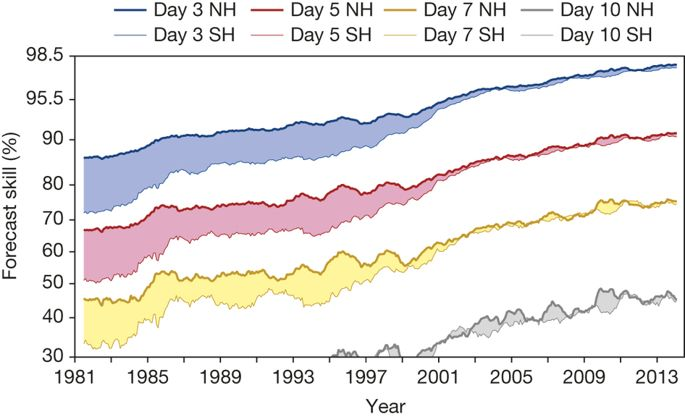
\includegraphics[width=0.8\textwidth]{figures/bauer_skill.jpg}

    \parencite{bauer}
  \end{figure}

\end{frame}

\note{
  Anomaly of 500 hPa geopotential height ECMWF (European Centre for Medium-Range Weather Forecasts)

  Gap between north and south due to lack of observations, bridged by satellites.


}
